\documentclass[a4paper, 12pt, table]{scrartcl}

% Use Hungarian Locale
\usepackage[magyar]{babel}

% Inputs
% Link between TeX and lua files
\usepackage{pyluatex}

% \begin{noindent}
\begin{python}
import sympy as sp
from sympy.printing.latex import LatexPrinter, print_latex
from sympy import latex
from python.calc import calculate

V = calculate({
    "code": {
        1: 1, 
        2: 1,
        3: 4,
        4: 2,
    },
    "name": "Sándor Tibor",
    "neptun": "C7XUDE"
})

N = V["numeric"]
P = V["parametric"]

from python.helper import printer, print_matrix, prin_TeX, my_latex

H = printer({
    "variables": V
})
\end{python}
% \end{noindent}

\usepackage{xargs}

\newcommand{\pv}[1]{\py{V["#1"]}}
\newcommand{\pvec}[2]{\py{V["#1"][#2]}}
\newcommand{\pmat}[3]{\py{V["#1"][#2, #3]}}

\newcommandx{\sipv}[3][3=]{\pyc{H["printSIVar"]({ "name":"#1", "unit":"#2", "dec":"#3" })}}
\newcommandx{\sipvec}[4][4=]{\pyc{H["printSIDirect"]({ "value":V["#1"][#2], "unit":"#3", "dec":"#4" })}}
\newcommandx{\sipmat}[5][5=]{\pyc{H["printSIDirect"]({ "value":V["#1"][#2, #3], "unit":"#4", "dec":"#5" })}}

% Figure and other imports
\usepackage{pdfpages}
\usepackage{standalone}

% Actual page layout
\usepackage[
  margin=20mm,
  footskip=12mm,
  headheight=20mm,
  % showframe
]{geometry}
\usepackage{fancyhdr}
\usepackage{lastpage}
\usepackage{hyperref}
\pagestyle{fancy}

\renewcommand\footrulewidth{1mm}
\renewcommand\headrulewidth{1mm}

\setlength\parindent{0em}
\setlength\parskip{.33em}

\setkomafont{disposition}{\color{red!40!black}\bfseries\sffamily}
\setkomafont{captionlabel}{\color{red!40!black}\bfseries\sffamily}

\fancyfoot[C]{\thepage\ / \pageref{LastPage}}
\fancyhead[L]{BMEGEMMBXVE, 2. SZHF}
\fancyhead[R]{%
  
\includegraphics[height = 12px]{static/signature.pdf}
  \py{V["name"]},
  \py{V["neptun"]}
}

% Math related stuff goes here
\usepackage{amsmath}
\usepackage{nccmath}
\usepackage{amssymb}
\usepackage{fontspec}
\usepackage{unicode-math}

% Set font to my liking
\setmainfont{TeX Gyre Termes}
\setsansfont[Scale=MatchUppercase]{TeX Gyre Heros}
\setmathfont{Asana Math}

% Variable printing according to Hungarian standards
\usepackage{icomma}
\usepackage{siunitx}
\sisetup{
  per-mode = symbol,
  locale=DE
}

% Slanted frac
\usepackage{xfrac}
% Derivatives
\usepackage{derivative}

% Math custom commands
\newcommand\iu{\mathbf{j}}
\newcommand{\rvec}[1]{\mathbfit{#1}}
\newcommand{\uvec}[1]{\widehat{\mathbfit{#1}}}
\newcommand{\rmat}[1]{\mathbf{#1}}
\newcommand{\spec}[1]{\mathfrak{#1}}

% Operator like commands
\DeclareMathOperator\atann{atan2}

% Switching between SI modes
\newcommand{\sifigures}[1]{\sisetup{round-mode=figures, round-precision=#1}}
\newcommand{\siplaces}[1]{\sisetup{round-mode=places, round-precision=#1}}
\newcommand{\sisci}{\sisetup{exponent-mode = scientific}}
\newcommand{\sifix}{\sisetup{exponent-mode = fixed}}

% Framed equations
\usepackage{mdframed}
% \begin{noindent}
\newenvironment{myframe}{%
\begin{mdframed}[%
backgroundcolor=gray!10,%
linecolor=red!40!black,%
linewidth=1mm,%
topline=false,%
rightline=false,%
bottomline=false,%
]\useshortskip}{\end{mdframed}}
% \end{noindent}

\usepackage{tikz}
\usepackage{pgfplots}
\pgfplotsset{compat=1.18, width=16cm, height=8.33cm}
\usepgfplotslibrary{fillbetween}
\pgfkeys{/pgf/number format/use comma}
\pgfkeys{/pgf/number format/1000 sep={\,}}
\pgfplotsset{%
  xmin=0,xmax=\lv{c}*1.05,
  every major tick/.style = {gray, semithick},
  axis x line=center,  axis y line=center,
  enlarge y limits=.05,
  axis line style={-to, thick},
  grid=both,
  grid style={line width=.1pt, draw=gray!20},
  major grid style={line width=.2pt,draw=gray!80},
  scaled y ticks=false,
}
\usetikzlibrary{
  calc,
  angles,
  quotes,
  backgrounds,
  patterns,
  arrows,
  arrows.meta,
  positioning,
  intersections,
  shapes.geometric,
}

\tikzset{
  dot/.style = {
      circle,
      fill=red!40!gray,
      minimum size=#1,
      draw=black,
      inner sep=0pt, outer sep=0pt,
      very thick,
    },
  dot/.default = 7pt,
  gdot/.style = {
      dot,
      fill=white
    },
  dim/.style = {
      latex-latex,
      draw=teal,
      ultra thick
    },
  joint/.style = {
      circle,
      draw=black,
      ultra thick,
      fill=cyan!20,
      minimum size=6.5mm,
      inner sep=0,
    },
  square/.style = {
      regular polygon,
      regular polygon sides=4
    },
  rod/.style = {
      rectangle,
      draw=black,
      minimum height=6mm,
      minimum width=6mm,
      fill=yellow!25,
      ultra thick,
      midway,
      outer sep=0,
    },
}

% Other included packages go here
\usepackage{tabto}
\usepackage{multicol}
\usepackage{xcolor}
\usepackage{float}
\usepackage{array}
\newcolumntype{x}[1]{>{\centering\arraybackslash\hspace{0pt}}p{#1}}
\newcolumntype{X}[1]{>{$}x{#1}<{$}}


% code: 1142
\begin{document}

\AddToShipoutPictureFG*{
  \setmainfont{Latin Modern Roman}
  \setmathfont{Latin Modern Math}
  \put(12cm,27.33cm){
    \makebox(7.5cm,1cm){
      \hfill \pv{name}
    }
  }
  \put(12cm,26.67cm){
    \makebox(7.5cm,1cm){
      \hfill \pv{neptun}
    }
  }
  \put(15.45cm,26cm){
    \makebox(7.5cm,1cm){
      \hfill 
\includegraphics[height=5mm]{./static/signature.pdf} \hfill
    }
  }

  \put(8.7cm,25cm){
    \makebox(17mm,0){\pvec{code}{1}}
    \makebox(12mm,0){\pvec{code}{2}}
    \makebox(15mm,0){\pvec{code}{3}}
    \makebox(12mm,0){\pvec{code}{4}}
  }

  \newcommand\com{\centering\scriptsize}
  \put(19.5mm, 53.2mm){
    \def\w{20.7mm}
    \makebox(\w,0){\com{}\sipmat{Delta_um}{0}{0}{}[4]}
    \makebox(\w,0){\com{}\sipmat{Delta_um}{1}{0}{}[4]}
    \makebox(\w,0){\com{}\sipmat{Delta_um}{2}{0}{}[4]}
    \makebox(\w,0){\com{}\sipmat{Delta_um}{3}{0}{}[4]}
    \makebox(\w,0){\com{}\sipmat{Delta_um}{4}{0}{}[4]}
    \makebox(\w,0){\com{}\sipmat{Delta_um}{5}{0}{}[4]}
    \makebox(\w,0){\com{}\sipmat{Delta_um}{6}{0}{}[4]}
    \makebox(\w,0){\com{}\sipmat{Delta_um}{7}{0}{}[4]}
  }
  \put(16.66mm, 44.6mm){
    \sisetup{drop-zero-decimal}
    \def\w{20.7mm}
    \makebox(\w,0){\com{}\sipmat{F_calc}{0}{0}{}[4]}
    \makebox(\w,0){\com{}\sipmat{F_calc}{2}{0}{}[4]}
    \makebox(\w,0){\com{}\sipmat{F_calc}{4}{0}{}[4]}
    \makebox(\w,0){\com{}\sipmat{F_calc}{6}{0}{}[4]}
    \makebox(\w,0){\com{}\sipmat{F_calc}{8}{0}{}[4]}
    \makebox(\w,0){\com{}\sipmat{F_calc}{10}{0}{}[4]}
    \makebox(\w,0){\com{}\sipmat{F_calc}{12}{0}{}[4]}
    \makebox(\w,0){\com{}\sipmat{F_calc}{14}{0}{}[4]}
  }
  \put(16.66mm, 36.2mm){
    \sisetup{drop-zero-decimal}
    \def\w{20.7mm}
    \makebox(\w,0){\com{}\sipmat{F_calc}{1}{0}{}[4]}
    \makebox(\w,0){\com{}\sipmat{F_calc}{3}{0}{}[4]}
    \makebox(\w,0){\com{}\sipmat{F_calc}{5}{0}{}[4]}
    \makebox(\w,0){\com{}\sipmat{F_calc}{7}{0}{}[4]}
    \makebox(\w,0){\com{}\sipmat{F_calc}{9}{0}{}[4]}
    \makebox(\w,0){\com{}\sipmat{F_calc}{11}{0}{}[4]}
    \makebox(\w,0){\com{}\sipmat{F_calc}{13}{0}{}[4]}
    \makebox(\w,0){\com{}\sipmat{F_calc}{15}{0}{}[4]}
  }
  \put(15.8mm, 27.1mm){
    \sisetup{drop-zero-decimal}
    \def\w{43mm}
    \makebox(\w,0){\com{}\sipmat{sigma_2}{0}{0}{}[4]}
    \makebox(\w,0){\com{}\sipmat{sigma_2}{1}{0}{}[4]}
    \makebox(\w,0){\com{}\sipmat{sigma_2}{2}{0}{}[4]}
    \makebox(\w,0){\com{}\sipvec{E_i}{0}{}[4]}
  }
}
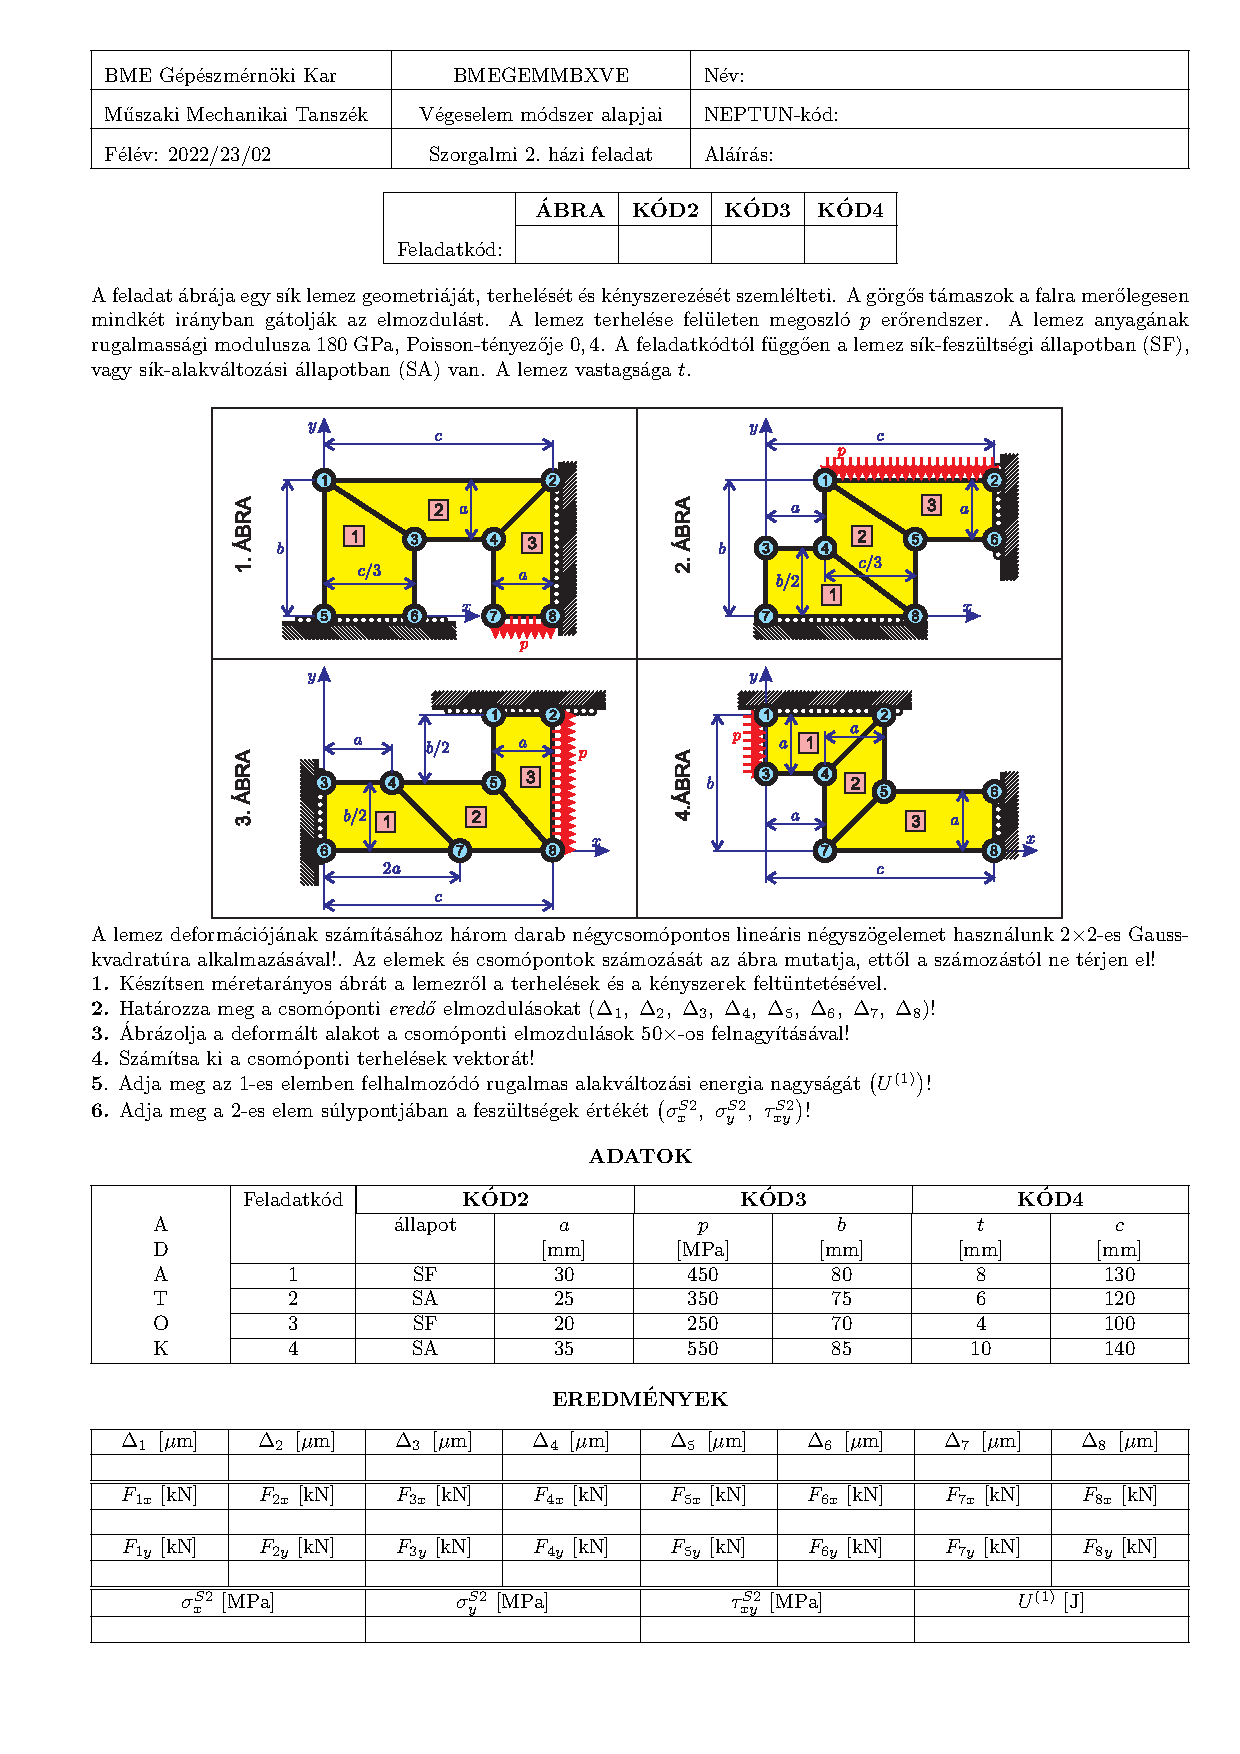
\includepdf[
  pages=-,
  scale=.95,
  pagecommand=\thispagestyle{fancy}
]{static/titlepage.pdf}
\setmainfont{TeX Gyre Termes}
\setmathfont{Asana Math}

\allowdisplaybreaks

% Section 1 -- fig
\section{Méretarányos ábra}

A feladatkódom (\texttt{\pvec{code}{1}\pvec{code}{2}\pvec{code}{3}\pvec{code}{4}})
alapján a szerkezetet jellemző adatok:
\begin{myframe}
  \vspace{-.66em}
  \begin{multicols}{2}
    \begin{itemize}
      \item \pyc{print(V["state"] == "SF" and "Sík-feszültségi" or "Sík-alakváltozási")} állapot,
      \item $p = \sipv{p}{MPa}$,
      \item $E = \sipv{E}{MPa}$,
      \item $\nu = \sipv{nu}{}$,

      \item $a = \sipv{a}{mm}$,
      \item $b = \sipv{b}{mm}$,
      \item $c = \sipv{c}{mm}$,
      \item $t = \sipv{t}{mm}$.
    \end{itemize}
  \end{multicols}
\end{myframe}

A megadott adatok alapján a lemezről készített méretarányos vázlat az
\ref{fig:construction}. ábrán látható. A lapon mért $\SI{.75}{cm}$ távolság
a valóságban $\SI{1}{cm}$-nek felel meg.

\begin{figure}[H]
  \centering
  \includestandalone{construction}
  \vspace{-2mm}
  \caption{Méretarányos ábra a lemezről}
  \vspace{-5mm}
  \label{fig:construction}
\end{figure}

\section{Csomóponti eredő elmozdulások}

\subsection{Általános adatok}

A csomópontok koordinátáit az \ref{table:U}. táblázat tartalmazza.
\begin{table}[H]
  \def\arraystretch{1.1}
  \centering
  \caption{A csomópontok koordinátái}
  % \begin{noindent}
  \begin{python}
print(r"\def\arraystretch{1.1}")
print(r"\begin{tabular}{| >{\cellcolor{gray!10}}{c} *{2}{|| X{1.5cm} | X{1.5cm}} |}")
print(r"\hline \rowcolor{yellow!10}")
print(r"Csp. & x & y & x \; [\text{mm}] & y \; [\text{mm}] \\")
print(r"\hline \hline")
for i in range(1, 9):
    print(
        f"{i} & {P[i]['x']} & {P[i]['y']} & " +
        f"{N[i]['x']:.0f} & {N[i]['y']:.0f} \\\\ \hline"
    )
print(r"\end{tabular}")
  \end{python}
  % \end{noindent}
  \label{table:U}
\end{table}

Az egyes elemekhez tartozó csomópontokat a \ref{table:lok}. táblázat foglalja
össze.
\begin{table}[H]
  \def\arraystretch{1.1}
  \centering
  \caption{Elem -- csomópont összerendelések}
  \begin{tabular}{| >{\cellcolor{gray!10}}{c} || c | c | c | c |}
    \hline
    \rowcolor{yellow!10}
    Elem & 1. csp                     & 2. csp                     & 3. csp                     & 4. csp                     \\ \hline \hline
    1    & \py{P["rectangles"][0][0]} & \py{P["rectangles"][0][1]} & \py{P["rectangles"][0][2]} & \py{P["rectangles"][0][3]} \\ \hline
    2    & \py{P["rectangles"][1][0]} & \py{P["rectangles"][1][1]} & \py{P["rectangles"][1][2]} & \py{P["rectangles"][1][3]} \\ \hline
    3    & \py{P["rectangles"][2][0]} & \py{P["rectangles"][2][1]} & \py{P["rectangles"][2][2]} & \py{P["rectangles"][2][3]} \\ \hline
  \end{tabular}
  \label{table:lok}
\end{table}

\subsection{Koordináta-transzformáció}

Mivel elemeink nem szabályos négyszögek, ezért a számítás megkönnyítéséhez
érdemes koordináta-transzformációt végrehajtani. Elemenként egy olyan lokális
$\xi$-$\eta$ koordináta-rendszerbe fogunk áttérni, ahol a lemezek csúcsainak
koordinátái rendre $(-1;-1)$, $(1;-1)$, $(1;1)$, $(-1;1)$. A két
koordináta-reprezentáció közötti kapcsolat:
\begin{myframe}
  \begin{equation}
    x = \sum_{i=1}^4 N_i \cdot x_i
    \text,
    \qquad
    \text{ és }
    \qquad
    y = \sum_{i=1}^4 N_i \cdot y_i
    \text,
  \end{equation}
\end{myframe}
ahol: $(x_i; y_i)$ az egyes csomópontok $x$-$y$ koordináta-rendszerbeli
koordinátája, $N_i$ pedig az $i$-edik formafüggvényt jelöli, melyek alakjai:
\begin{myframe}
  \begin{gather}
    N_1 = \frac{1}{4} (1 - \xi) (1 - \eta) \text, \\
    N_2 = \frac{1}{4} (1 + \xi) (1 - \eta) \text, \\
    N_3 = \frac{1}{4} (1 + \xi) (1 + \eta) \text, \\
    N_4 = \frac{1}{4} (1 - \xi) (1 + \eta) \text.
  \end{gather}
\end{myframe}
Ezek alapján felírható az egyes elemekhez tartozó lokális és a globális
koordináta-rendszerek közötti transzformáció:
\begin{myframe}
  \begin{alignat}{9}
     & (1) \qquad & \rightarrow \qquad x & = \py{my_latex(V["transform"][0]["x"],2)} \text, &  & \qquad y = \py{my_latex(V["transform"][0]["y"],2)}
    \\
     & (2) \qquad & \rightarrow \qquad x & = \py{my_latex(V["transform"][1]["x"],2)} \text, &  & \qquad y = \py{my_latex(V["transform"][1]["y"],2)}
    \\
     & (3) \qquad & \rightarrow \qquad x & = \py{my_latex(V["transform"][2]["x"],2)} \text, &  & \qquad y = \py{my_latex(V["transform"][2]["y"],2)}
  \end{alignat}
\end{myframe}
A leképezés inverze pedig:
\begin{myframe}
  \begin{alignat}{9}
     & (1) \qquad & \rightarrow \qquad \xi & = \py{my_latex(V["transform"][0]["xi"], 4)} \text, &  & \qquad \eta = \py{my_latex(V["transform"][0]["eta"], 4)}
    \\
     & (2) \qquad & \rightarrow \qquad \xi & = \py{my_latex(V["transform"][1]["xi"], 4)} \text, &  & \qquad \eta = \py{my_latex(V["transform"][1]["eta"], 4)}
    \label{eq:alma}
    \\
     & (3) \qquad & \rightarrow \qquad \xi & = \py{my_latex(V["transform"][2]["xi"], 4)} \text, &  & \qquad \eta = \py{my_latex(V["transform"][2]["eta"], 4)}
  \end{alignat}
\end{myframe}

\subsection{A Jacobi-mátrixok}

Írjuk fel az egyes elemekhez tartozó leképezések Jacobi-mátrixát. Ehhez először
A formafüggvények $\xi$ és $\eta$ szerinti parciális deriváltakra van szükségünk:
\begin{myframe}
  \begin{alignat}{9}
    \pdv{N_1}{\xi}  & = \frac{\eta - 1}{4}
    \text, \qquad \quad
    \pdv{N_2}{\xi}  & = \frac{-\eta + 1}{4}
    \text, \qquad \quad
    \pdv{N_3}{\xi}  & = \frac{\eta + 1}{4}
    \text, \qquad \quad
    \pdv{N_4}{\xi}  & = \frac{-\eta - 1}{4}
    \text,                                  \\[3mm]
    \pdv{N_1}{\eta} & = \frac{\xi - 1}{4}
    \text, \qquad \quad
    \pdv{N_2}{\eta} & = \frac{-\xi - 1}{4}
    \text, \qquad \quad
    \pdv{N_3}{\eta} & = \frac{\xi + 1}{4}
    \text, \qquad \quad
    \pdv{N_4}{\eta} & = \frac{-\xi + 1}{4}
    \text.
  \end{alignat}
\end{myframe}
A Jacobi mátrix alakja paraméteresen:
\begin{myframe}
  \begin{equation}
    \rmat J_i = \begin{bmatrix}
      \displaystyle \pdv{x}{\xi}  &
      \displaystyle \pdv{y}{\xi}    \\[4mm]
      \displaystyle \pdv{x}{\eta} &
      \displaystyle \pdv{y}{\eta}   \\
    \end{bmatrix} = \begin{bmatrix}
      \displaystyle \sum \pdv{N_i}{\xi} x_i  &
      \displaystyle \sum \pdv{N_i}{\xi} y_i    \\[4mm]
      \displaystyle \sum \pdv{N_i}{\eta} x_i &
      \displaystyle \sum \pdv{N_i}{\eta} y_i   \\
    \end{bmatrix}
    \text.
  \end{equation}
\end{myframe}
Ezek alapján az egyes elemekhez tartozó Jacobi-mátrixok numerikus alakja:
\begin{myframe}
  \begin{align}
    \rmat J_1 & =
    \py{my_latex(V["J"][0], -1, mat_str="array").replace('cc', "*{2}{X{3cm}}")}
    \text,
    \\
    \rmat J_2 & =
    \py{my_latex(V["J"][1], -1, mat_str="array").replace('cc', "*{2}{X{3cm}}")}
    \text,
    \\
    \rmat J_3 & =
    \py{my_latex(V["J"][2], -1, mat_str="array").replace('cc', "*{2}{X{3cm}}")}
    \text.
  \end{align}
\end{myframe}
A formafüggvények globális és lokális koordináták szerinti parciális deriváltai
között a Jacobi-mát\-rix\-ok inverzei teremtenek kapcsolatot:
\begin{myframe}
  \begin{equation}
    \begin{bmatrix}
      \displaystyle \pdv{N_i}{x} \\[4mm]
      \displaystyle \pdv{N_i}{y} \\
    \end{bmatrix}
    =
    \underbrace{
      \begin{bmatrix}
        \displaystyle \pdv{\xi}{x} &
        \displaystyle \pdv{\eta}{x}  \\[4mm]
        \displaystyle \pdv{\xi}{y} &
        \displaystyle \pdv{\eta}{y}  \\
      \end{bmatrix}
    }_{\rmat J^{-1}}
    \begin{bmatrix}
      \displaystyle \pdv{N_i}{\xi}  \\[4mm]
      \displaystyle \pdv{N_i}{\eta} \\
    \end{bmatrix}
    \text.
  \end{equation}
\end{myframe}
Ezek paraméteresen:
\begin{myframe}
  \def\arraystretch{2.15}
  \begin{align}
    {\rmat J_1}^{-1} & =
    \py{my_latex(V["inv_J"][0], 4, mat_str="array").replace('cc', "*{2}{X{4cm}}")}
    \text,
    \\
    {\rmat J_2}^{-1} & =
    \py{my_latex(V["inv_J"][1], 4, mat_str="array").replace('cc', "*{2}{X{4cm}}")}
    \text,
    \\
    {\rmat J_3}^{-1} & =
    \py{my_latex(V["inv_J"][2], 4, mat_str="array").replace('cc', "*{2}{X{4cm}}")}
    \text.
  \end{align}
\end{myframe}

\subsection{Elemi merevségi mátrixok}

Tetszőleges síkbeli négyszögelem merevségi mátrixa az alábbi összefüggéssel
számítható:
\begin{myframe}
  \begin{equation}
    \rmat K_i
    = \int_{-1}^{+1} \int_{-1}^{+1}
    \rmat B^{\mathsf T}_i \,
    \rmat D_i \,
    \rmat B_i \,
    t \,
    \det \rmat J_i \,
    \mathrm d \xi \,
    \mathrm d \eta
    \text.
  \end{equation}
\end{myframe}

Az határozott integrál értéket $2 \times 2$-es Gauss-kvadratúra segítségével
fogjuk közelíteni:
\begin{myframe}
  \begin{equation}
    \rmat K_i \approx
    \sum_{i=1}^{2} \sum_{j=1}^{2}
    w_i \,
    w_j \,
    \rmat B^{\mathsf T}_i \,
    \rmat D_i \,
    \rmat B_i \,
    t \,
    \det \rmat J_i \,
    \text,
  \end{equation}
\end{myframe}

Az integrálási súlyok esetünkben: $w_1 = w_2 = 1$. A Gauss-pontok koordinátáit
pedig a \ref{fig:Gaussian}. ábra tartalmazza.
\begin{figure}[H]
  \centering
  \begin{tikzpicture}[thick, scale=3]
    \draw[draw=gray, fill=gray!10] (-1,-1) rectangle (1,1);
    \draw[ultra thick, -to] (-1.2,0) -- ++(2.5,0) node[below left] {$\xi$};
    \draw[ultra thick, -to] (0,-1.2) -- ++(0,2.5) node[below right] {$\eta$};

    % \node[dot] (t) at (-0.58, -.58) {}; \node[above right] at (t) {$(\xi_1; \eta_1)$}; \node[below left]  at (t) {$(-1/\sqrt{3}; -1/\sqrt{3})$};
    % \node[dot] (t) at (+0.58, -.58) {}; \node[above left]  at (t) {$(\xi_2; \eta_1)$}; \node[below right] at (t) {$( 1/\sqrt{3}; -1/\sqrt{3})$};
    % \node[dot] (t) at (+0.58, +.58) {}; \node[below left]  at (t) {$(\xi_2; \eta_2)$}; \node[above right] at (t) {$( 1/\sqrt{3};  1/\sqrt{3})$};
    % \node[dot] (t) at (-0.58, +.58) {}; \node[below right] at (t) {$(\xi_1; \eta_2)$}; \node[above left]  at (t) {$(-1/\sqrt{3};  1/\sqrt{3})$};

    \node[dot] (t) at (-0.58, -.58) {}; \node[below left,  xshift=4mm ] at (t) {$(-1/\sqrt{3}; -1/\sqrt{3}) = (\xi_1; \eta_1)$};
    \node[dot] (t) at (+0.58, -.58) {}; \node[below right, xshift=-4mm] at (t) {$(\xi_2; \eta_1) = ( 1/\sqrt{3}; -1/\sqrt{3})$};
    \node[dot] (t) at (+0.58, +.58) {}; \node[above right, xshift=-4mm] at (t) {$(\xi_2; \eta_2) = ( 1/\sqrt{3};  1/\sqrt{3})$};
    \node[dot] (t) at (-0.58, +.58) {}; \node[above left,  xshift=4mm ] at (t) {$(-1/\sqrt{3};  1/\sqrt{3}) = (\xi_1; \eta_2)$};
  \end{tikzpicture}
  \caption{Gauss-pontok szemléltelése}
  \label{fig:Gaussian}
\end{figure}

A képletben szerepel egy $\rmat B$ mátrix is, amely a formafüggvények $x$ és $y$
változók szerinti parciális deriváltjait tartalmazza az alábbi módon:
\begin{myframe}
  \newcommand{\nd}[2]{\displaystyle\pdv{N_{#1}}{#2}}
  \def\arraystretch{2}
  \begin{equation}
    \rmat B_i = \begin{bmatrix}
      \nd{1}{x} & 0         &
      \nd{2}{x} & 0         &
      \nd{3}{x} & 0         &
      \nd{4}{x} & 0
      \\
      0         & \nd{1}{y} &
      0         & \nd{2}{y} &
      0         & \nd{3}{y} &
      0         & \nd{4}{y}
      \\
      \nd{1}{y} & \nd{1}{x} &
      \nd{2}{y} & \nd{2}{x} &
      \nd{3}{y} & \nd{3}{x} &
      \nd{4}{y} & \nd{4}{x}
      \text.
    \end{bmatrix}
  \end{equation}
\end{myframe}

A $\rmat D$ mátrix pedig
\py{V["state"] == "SF" and "sík-feszültségi" or "sík-alakváltozási"} állapot
esetén az alábbi alakot veszi fel:
\begin{myframe}
  \newcommand{\sfa}[2]{\py{V["state"] == "SF" and r"#1" or r"#2"}}
  \def\arraystretch{1.15}
  \begin{equation}
    \rmat D_i =
    \sfa{\frac{E}{1 - \nu^2}}{\frac{E}{(1+\nu)(1-2\nu)}} \;
    \left[\begin{array}{*{3}{X{15mm}}}
        \sfa{1}{1-\nu} & \nu            & 0                         \\
        \nu            & \sfa{1}{1-\nu} & 0                         \\
        0              & 0              & \sfa{(1-\nu)}{(1-2\nu)}/2
      \end{array}\right]
    \text.
  \end{equation}
\end{myframe}

Az elemi merevségi mátrixok tehát numerikusan:
\begin{myframe}
  \begin{align}
    \siplaces{4}
    \sifix{}
    \rmat K_1 = \left[
      \scalebox{.75}{$\begin{array}{*{8}{X{1.55cm}}}
                            \pyc{print_matrix(V["K_i"][0], 1e-6, 1e-6)}
                          \end{array}$}
      \right]
    \cdot 10^6
    \\
    \siplaces{4}
    \sifix{}
    \rmat K_2 = \left[
      \scalebox{.75}{$\begin{array}{*{8}{X{1.55cm}}}
                            \pyc{print_matrix(V["K_i"][1], 1e-6, 1e-6)}
                          \end{array}$}
      \right]
    \cdot 10^6
    \\
    \siplaces{4}
    \sifix{}
    \rmat K_3 = \left[
      \scalebox{.75}{$\begin{array}{*{8}{X{1.55cm}}}
                            \pyc{print_matrix(V["K_i"][2], 1e-6, 1e-6)}
                          \end{array}$}
      \right]
    \cdot 10^6
  \end{align}
\end{myframe}

\subsection{A globális merevségi mátrix}

A globális merevségi mátrix meghatározásához írjuk fel az egyes elemekhez tartozó szabadsági foko-
kat mátrixosan:
\begin{myframe}
  \begin{equation}
    \rmat{DOF} =
    \py{latex(sp.Matrix(V["DOF"]), mat_str="array").replace("cccccccc", "*{8}{X{7mm}}")}
    \text.
  \end{equation}
\end{myframe}

A globális merevségi mátrix összeállításakor figyelnünk kell arra, hogy az adott
elem merevségi mátrixának megfelelő elemeit a hozzá tartozó szabadsági fokhoz
tartozó helyhez rendeljük hozzá. Ezt a \ref{fig:K-construction} ábra
szemlélteti.
\begin{figure}[ht]
  \centering
  \includestandalone{K-construction}
  \caption{A globális merevségi mátrix szemléletes felépítése}
  \label{fig:K-construction}
\end{figure}

A globális merevségi mátrix tehát az alábbi alakot veszi fel:
\begin{myframe}
  \begin{equation}
    \siplaces{4}
    \sifix{}
    \rmat K = \left[
      \scalebox{.45}{
        $\begin{array}{*{16}{X{1.45cm}}}
            \pyc{print_matrix(V["K"], 1e-6, 1e-6)}
          \end{array}$
      }
      \right]
    \cdot 10^6
    \text.
  \end{equation}
\end{myframe}

\subsection{A merevségi egyenlet}

Írjuk fel a globális elmozdulás-vektort. A görgős megtámasztás miatt a
(\py{P["F"]["x"][0]})-es és a (\py{P["F"]["x"][1]})-os pontokban az $x$,
az (\py{P["F"]["y"][0]})-ös és a (\py{P["F"]["y"][1]})-os pontokban pedig az
$y$ irányú elmozdulás gátolt, vagyis ezen elmozdulás-komponensek zérusak.
Ezek alapján a vektor paraméteresen:
\begin{myframe}
  \begin{equation}
    \rvec U = \py{latex(V["U_sym"].T)}^{\mathsf T}
    \text.
  \end{equation}
\end{myframe}

A görgős támasz miatt a gátolt irányokban kényszererők ébrednek, valamint
a megoszló terhelés, mint koncentrált erő is megjelenik a globális
terhelésvektorban, amely az alábbi alakot veszi fel:
\begin{myframe}
  \begin{equation}
    \rvec F = \py{my_latex(V["F_sym"].T, fold_short_frac=True)}^{\mathsf T}
    \text.
  \end{equation}
\end{myframe}

A rendszer merevségi egyenlete:
\begin{equation}
  \rmat K \rvec U = \rvec F
  \text.
\end{equation}

Fontos, hogy a merevségi egyenlet csak abban az esetben oldható meg mátrix
inverziós módszerrel, amennyiben $\rmat K$ mátrix reguláris. Mivel ez a
feltétel nem teljesül, ezért az egyenletrendszert kondenzálnunk kell.
A kondenzált merevségi egyenletrendszert úgy kapjuk meg, hogy a gátolt
szabadsági fokokhoz tartozó sorokat és oszlopokat töröljük az eredeti, globális
merevségi egyenletből:
\begin{myframe}
  \begin{equation}
    \sifix{}
    \siplaces{4}
    \underbrace{\left[
        \scalebox{.48}{
          $\begin{array}{*{12}{X{1.45cm}}}
              \pyc{print_matrix(V["K_kond"], 1e-16, 1e-6)}
            \end{array}$
        }
        \right]
      \cdot 10^6}_{\widehat{\rmat K}}
    \cdot
    \underbrace{\left[
    \scalebox{.48}{
    $\py{latex(V["U_sym_kond"], mat_delim="").replace('cc', "X{5mm}X{4.95mm}")}$
    }
    \right]}_{\widehat{\rvec U}}
    \siplaces{0}
    =
    \underbrace{\left[
        \scalebox{.48}{
          $\begin{array}{*{12}{X{1.45cm}}}
              \pyc{print_matrix(V["F_kond"])}
            \end{array}$
        }
        \right]}_{\widehat{\rvec F}}
    \text.
  \end{equation}
\end{myframe}

Mivel $\widehat{\rmat K}$ mátrix reguláris, ezért az egyenletrendszer
mátrix-invertálással megoldható, vagyis:
\begin{myframe}
  \begin{equation}
    \widehat{\rvec U}
    =
    \sifix{}
    \siplaces{4}
    \underbrace{\left[
        \scalebox{.5}{
          $\begin{array}{*{12}{X{1.45cm}}}
              \pyc{print_matrix(V["K_kond_inv"], 1e-16, 1e+6)}
            \end{array}$
        }
        \right]
      \cdot 10^{-6}}_{\widehat{\rmat K}^{-1}}
    \cdot
    \siplaces{0}
    \underbrace{\left[
        \scalebox{.5}{
          $\begin{array}{*{12}{X{1.45cm}}}
              \pyc{print_matrix(V["F_kond"])}
            \end{array}$
        }
        \right]}_{\widehat{\rvec F}}
    \text.
  \end{equation}
\end{myframe}

Az egyenlet megoldása numerikusan:
\begin{myframe}
  \begin{equation}
    \siplaces{6}
    \widehat{\rvec U} = \left[
      \scalebox{.65}{
        $\begin{array}{c}
            \pyc{print_matrix(V["U_kond"])}
          \end{array}$
      }
      \right]
    \text{mm}
    \text.
  \end{equation}
\end{myframe}

A globális elmozdulásvektorba visszahelyettesítve:
\begin{myframe}
  \begin{equation}
    \siplaces{6}
    \rvec U = \left[
      \scalebox{.65}{
        $\begin{array}{c}
            \pyc{print_matrix(V["U_calc"])}
          \end{array}$
      }
      \right]
    \text{mm}
    \text.
  \end{equation}
\end{myframe}

Az eredő elmozdulások a Pitagorasz-tétel alapján számíthatóak:
\begin{myframe}
  \begin{equation}
    \Delta_i = \sqrt{{U_i}^2 + {V_i}^2}
    \text.
  \end{equation}
\end{myframe}

Numerikusan:
\begin{myframe}
  \begin{equation}
    \rvec{\Delta} = \begin{bmatrix}
      \Delta_1 \\
      \Delta_2 \\
      \Delta_3 \\
      \Delta_4 \\
      \Delta_5 \\
      \Delta_6 \\
      \Delta_7 \\
      \Delta_8 \\
    \end{bmatrix}
    =
    \siplaces{6}
    \begin{bmatrix}
      \pyc{print_matrix(V["Delta_mm"])}
    \end{bmatrix}
    \text{mm}
    =
    \siplaces{3}
    \begin{bmatrix}
      \pyc{print_matrix(V["Delta_um"])}
    \end{bmatrix}
    \upmu\text{m}
    \text.
  \end{equation}
\end{myframe}

\section{A deformált alak ábrázolása}

A szerkezet deformált alakját a \ref{fig:deformed}. ábra szemlélteti.
Az elmozdulások 50-szeres nagyítással vannak feltüntetve.

\begin{figure}[H]
  \centering
  \vspace{-5mm}
  \includestandalone{deformed}
  \vspace{-2mm}
  \caption{A deformált alak ábrázolása}
  \vspace{-5mm}
  \label{fig:deformed}
\end{figure}

\section{A csomóponti terhelések vektora}

A globális terhelési vektor a merevségi egyenlet alapján:
\begin{myframe}
  \begin{equation}
    \rvec F
    = \rmat K \rvec U
    =
    \siplaces{2} \sisetup{drop-zero-decimal}
    \underbrace{\left[
        \scalebox{.667}{$\begin{array}{c}
              \pyc{print_matrix(V["F_calc"], 1e-6, 1, 2)}
            \end{array}$}
        \right]}_{\rvec F}
    \mathrm N
    = \siplaces{0}
    \underbrace{\left[
        \scalebox{.667}{$\begin{array}{c}
              \pyc{print_matrix(V["F_base"], 1e-6, 1, 0)}
            \end{array}$}
        \right]}_{\rvec F_t \text{ -- terhelés}}
    \mathrm N
    + \siplaces{2}
    \underbrace{\left[
        \scalebox{.667}{$\begin{array}{c}
              \pyc{print_matrix(V["F_reac"], 1e-6, 1, 2)}
            \end{array}$}
        \right]}_{\rvec F_r \text{ -- reakció}}
    \mathrm N
    \text.
  \end{equation}
\end{myframe}

A csomóponti terhelések vektorának nemzérus komponensei tehát:
\begin{myframe}
  \vspace{-.66em}
  \begin{multicols}{3}
    \begin{itemize}
      % \begin{noindent}
      \begin{python}
j = 0
for i in range(16):
    if abs(V["F_calc"][i, 0]) >= 1:
        j += 1
        print(
            r"\item $F_{" + str(i // 2 + 1) + 
            (i % 2 and "y" or "x") + 
            r"} = ", end=""
        )
        prin_TeX(V["F_calc"][i, 0] / 1000, "kN", 3)
        print("$" + (j == 6 and "." or ","))
      \end{python}
      % \end{noindent}
    \end{itemize}
  \end{multicols}
\end{myframe}

\clearpage
\section{Az (1)-es elemben tárolt rugalmas alakváltozási energia}

Egy tetszőleges elemben ébredő rugalmas alakváltozási energia az alábbi
képlettel határozható meg:
\begin{myframe}
  \begin{equation}
    U_i = \frac{1}{2} \rvec U_i^{\mathsf T} \rmat K_i \rvec U_i
    \text.
  \end{equation}
\end{myframe}
A képletben $\rvec U_i$ a lokális elmozdulás-vektort, $\rmat K_i$ pedig az
elemhez tartozó merevségi mátrixot jelöli. Az (1)-es elemben felhalmozódó
rugalmas alakváltozási energia ezek alapján:
\begin{myframe}
  \begin{equation}
    U_1
    = \frac{1}{2} \rvec U_1^{\mathsf T} \rmat K_1 \rvec U_1
    = \pyc{prin_TeX(V["E_i"][0], "J", 4)}
    \text.
  \end{equation}
\end{myframe}

\section{A (2)-es elem súlypontjában ébredő feszültségek}

Egy elem tetszőleges pontjában ébredő feszültségek az alábbi képlettel
számítható:
\begin{myframe}
  \begin{equation}
    \rvec \sigma_i(\xi; \eta)
    = \rmat D \, \rmat B_i(\xi; \eta) \rvec U_i
    \text.
  \end{equation}
\end{myframe}
Mivel a (2)-es elem súlypontjában vagyunk kíváncsiak a feszültségek értékeire,
ezért először meg kell határoznunk ennek koordinátáit. Ezek a globális
koordináta-rendszerben az alábbi formulával határozhatóak meg:
\begin{myframe}
  \begin{equation}
    x_s = \frac{1}{6A}\sum _{i=1}^{4}(x_{i}+x_{i+1})(x_{i}\ y_{i+1}-x_{i+1}\ y_{i})
    \text,
    \qquad
    y_s = \frac{1}{6A}\sum _{i=1}^{4}(y_{i}+y_{i+1})(x_{i}\ y_{i+1}-x_{i+1}\ y_{i})
    \text,
  \end{equation}
\end{myframe}
ahol $A_i$ a négyszög előjeles területe, értéke az alábbi képlettel számítható:
\begin{myframe}
  \begin{equation}
    A_i = \frac{1}{2}\sum _{i=1}^{4}(x_{i}\ y_{i+1}-x_{i+1}\ y_{i})
  \end{equation}
\end{myframe}
A fenti kifejezésekbe $i=4$ esetén adódó $i + 1 = 5$-ödik elemek helyére az
első elemhez tartozó mennyiségeket kell behelyettesíteni. A (2)-es elem
súlypontja a globális koordináta rendszerben:
\begin{myframe}
  \begin{equation}
    x_s = \pyc{prin_TeX(V["C"][1]["x"], "mm", 4)}
    \text,
    \qquad
    y_s = \pyc{prin_TeX(V["C"][1]["y"], "mm", 4)}
    \text.
  \end{equation}
\end{myframe}
A (\ref{eq:alma})-es egyenlet segítségével a súlypont koordinátái a lokális
koordináta-rendszerben:
\begin{myframe}
  \begin{equation}
    \sisetup{drop-zero-decimal}
    \xi_s = \pyc{prin_TeX(V["C"][1]["xi"], "", 4)}
    \text,
    \qquad
    \eta_s = \pyc{prin_TeX(V["C"][1]["eta"], "", 4)}
    \text.
  \end{equation}
\end{myframe}
A (2)-es elem súlypontjában ébredő feszültségek tehát:
\begin{myframe}
  \begin{equation}
    \rvec \sigma_2(\xi_s; \eta_s)
    =
    \begin{bmatrix}
      \sigma_x \\ \sigma_y \\ \tau_{xy}
    \end{bmatrix}
    =
    \siplaces{4}
    \begin{bmatrix}
      \pyc{print_matrix(V["sigma_i"][1])}
    \end{bmatrix}
    \mathrm{MPa}
    \text.
  \end{equation}
\end{myframe}


\clearpage
\tableofcontents

\vfill

\section*{Felhasznált szoftverek}

\begin{itemize}
  \item \href{https://neovim.io}{\texttt{Neovim}}
        \tabto{3.9cm} – \tabto{4.7cm}
        Open Source szövegszerkesztő

  \item \texttt{Lua\LaTeX}
        \tabto{3.9cm} – \tabto{4.7cm}
        \LaTeX{} fordító

  \item \texttt{Ti\textit{k}Z}
        \tabto{3.9cm} – \tabto{4.7cm}
        Vektorgrafika

  \item \texttt{python}
        \tabto{3.9cm} – \tabto{4.7cm}
        Számítások elvégzése
\end{itemize}

A házi feladat teljes forráskódja -- beleértve a számolást és dokumentációt --
megtekinthető az alábbi linken:
\texttt{\href{https://github.com/tibi1220/VEM-2SZHF}{https://github.com/tibi1220/VEM-2SZHF}}

\end{document}
